\documentclass[11pt]{article}

\usepackage{hyperref}
\usepackage{graphicx}
\usepackage{xcolor}

%opening
\title{Saddle Point Problems or Min-Max Problems}
\date{}
\author{
	Pavlenko, Nikolay\\
	\texttt{n.pavlenko@innopolis.university}
	\and
	Dyussenova, Ashera\\
	\texttt{a.dyussenova@innopolis.university}
}

\begin{document}

\maketitle

\section*{Introduction:}

Saddle point or min-max problems are more difficult problems than minimization problems. Meanwhile, min-max problems often arise in machine learning. The goal of this project is to understand the difference between min-max problems and minimization problems, and to learn methods for min-max problems. \\

This project is built upon an analysis of two papers: \href{https://openreview.net/pdf?id=r1laEnA5Ym}{\textbf{A Variational Inequality Perspective on Generative Adversarial Networks}} and \href{https://proceedings.neurips.cc/paper/2019/file/4625d8e31dad7d1c4c83399a6eb62f0c-Paper.pdf}{\textbf{On the Convergence of Single-Cell Stochastic Extra-Gradient Methods}}.

In order to comply with the requirement to have a single \LaTeX\ file in the root directory of the project, this file will cover detailed analysis of both papers, though they will be contained in separate sections. Analysis of the problem in general and conclusion will follow the rest of the report in the final section of the .tex file.

\section{A Variational Inequality Perspective on Generative Adversarial Networks:}

	\subsection{Problem Statement:}
	Authors of the paper want to achieve a more stable and reliable training process for Generative adversarial networks (GANs). In pursuit of that goal they reformulate the GAN objective as a two-player game in the sense of game theory, and they address that game as a variational inequality problem (VIP). VIP framework encompasses traditional saddle-point optimization algorithms, so it is relevant towards our investigation of min-max problems. \\
	
	Once the GAN optimization problem is reformulated as VIP, the goal is to find the optimal set $\Omega$ that would verify the following equality: 
	$$
	\textrm{find } \omega^*\in\Omega \textrm{ such that } F(\omega^*)^T(\omega-\omega^*)\geq0,\textrm{ } \forall\omega\in\Omega,
	$$
	where $\omega=(\theta,\varphi),$  $\omega^*=(\theta^*,\varphi^*),$ $\Omega=\Theta\times\Phi,$ $F(\omega)=[\nabla_{\theta}\mathcal{L}_G(\theta,\varphi)\textrm{ }\nabla_{\varphi}\mathcal{L}_D(\theta,\varphi)]^T$. $G$, $D$ are respectively generator and discriminator in GAN, $(\theta,\varphi)$ are parameters of $D$ and $G$, $(\theta^*,\varphi^*)$ is a stationary point (non-negative gradient in any direction).
	
	\subsection{Main Idea of the Approach:}
	
	Main idea of the \textit{extrapolation from the past} technique is to optimize the existing \textit{extrapolation} technique by storing and re-using the extrapolated gradient, thereby requiring only one computation of the gradient per update, rather than two: \\
	\textbf{Standard extrapolation:}
	$$
	\textrm{Compute extrapolated point: }\omega_{t+1/2}=P_{\Omega}[\omega_t-\eta F(\omega_{t-1/2})] $$
	$$
	\textrm{Perform update step: }\omega_{t+1}=P_{\Omega}[\omega_t-\eta F(\omega_{t+1/2})]\textrm{ and store: }F(\omega_{t+1/2})
	$$
	\textbf{Extrapolation from the past:}
	$$
	\textrm{Compute extrapolated point: }\omega_{t+1/2}=P_{\Omega}[\omega_t-\eta F(\omega_t)]
	$$
	$$
	\textrm{Perform update step: }\omega_{t+1}=P_{\Omega}[\omega_t-\eta F(\omega_{t+1/2})]
	$$
	
	\subsection{Theory and Background:}
		
		\subsubsection{Related Work:}
		There are a multitude of VIP optimization methods studied in literature, which the authors used in order to develop their own. Two standard methods are the \textit{gradient method}(Bruck, 1977) and the \textit{extragradient method} (Korpelevich, 1976). More recent methods use \textit{uniform average} in \textit{averaging} techniques(Nedi\'c and Ozdaglar, 2009), which guarantees convergence for any bounded monotone operator with a $O(1/\sqrt{t})$ rate, and \textit{extragradient method} (Nesterov, 2007), which does not require averaging and converges at an even faster rate of $O(1/t)$. \\
		
		The main idea that was discovered by the authors of the paper in relation to VIP - \textit{extrapolation from the past} was also already discovered previously by Chiang et al. (2012, Alg. 1) for general online learning.
		
		\subsubsection{Theoretical Framework:}
		In their work the authors use concepts from multiple different fields. Most importantly, they view the training of a GAN as a variational inequality, where the generator and discriminator aim to perform optimization in a game theory setting. They also cover stochastic optimization in their work, which was not done by many of the authors who preceded them. The solution presented in this paper is also dependent on stochastic gradient descent with averaging, extrapolation and extrapolation from the past.
		
		\subsubsection{Key Features:}
		\begin{itemize}
			\item The solution presented by the authors is guaranteed to sublinearly converge in most cases, unlike some of the older methods that were also covered in the paper.
			\begin{figure}[h]
				\centering
				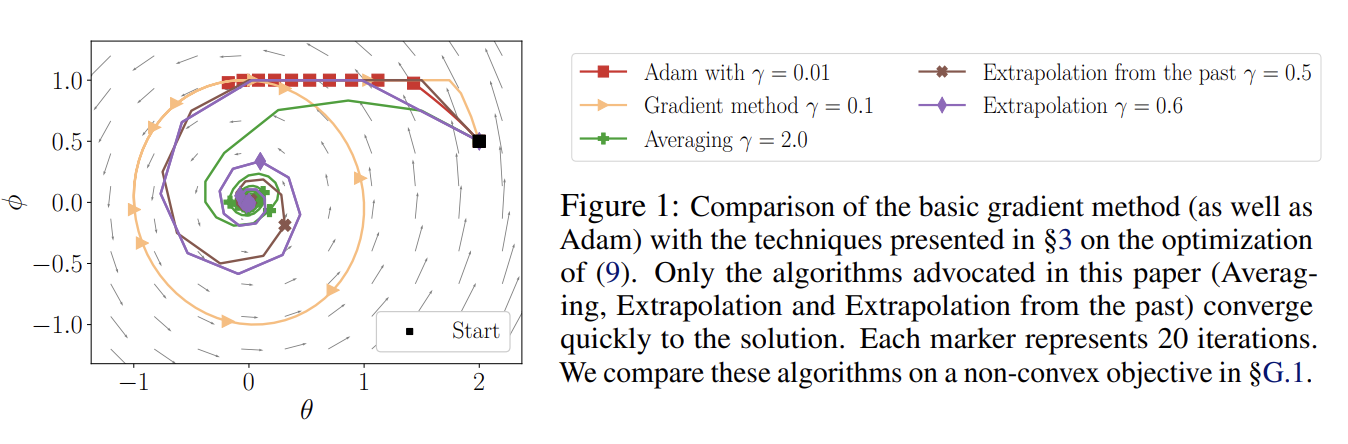
\includegraphics[scale=0.7]{pictures/pic2.png}
				\label{fig:labe}
			\end{figure}
			\item Recognizing that GANs involve stochastic gradients computed on mini-batches of data, the solution accounts for the inherent randomness and uncertainty in the optimization process, differing from previous work on the subject.
			\item The solution is not limited to a single type of GAN, and can be used with any architecture of the model of that type, making it versatile and widely applicable.
		\end{itemize}
		
		\subsubsection{Causes behind Good Performance:}
		Several factors are worth mentioning when talking about good performance of the solution:
		\begin{itemize}
			\item Solution guarantees fewer computations per iteration when compared to original extrapolation solution, so it is by definition more computationally efficient.
			\item It is based upon an existing solution that was proven to work well, so as an improvement on it it is also guaranteed to perform at least as well.
			\item It handles stochastic gradients, which makes it exceptionally well-suited for the purpose of GAN training. 
		\end{itemize}
		
		\subsubsection{Improvements over Older Methods:}
		Authors of the paper introduce a novel technique: \textit{extrapolation from the past}. Its improvement over the older \textit{extrapolation} technique is in requiring only one gradient descent computation per update, rather than two. \\
		Furthermore, their newly-developed techniques achieve a $4-6\%$ better inception score and the Fr\'echet inception distance than Miyato et al. (2018), while using CIFAR-10 dataset with a WGAN-GP and a ResNet generator.
	
	\subsection{Essence of Proof:}
	
	The essence of the proof for the method proposed in the paper lies in providing rigorous mathematical guarantees that the optimization algorithms will converge to a solution in the context of GAN training. The proof also relies on several assumptions: that function $F$ is strongly monotone and L-Lipschitz. If those assumptions are not fulfilled, then standard extrapolation technique has to be used, as it is guaranteed to converge linearly for a bilinear game.
	
	\subsection{Experiments and Results:}
	Authors structured their experiments in the following way: they compared the following optimization algorithms: baselines are SGD and Adam using either simultaneous updates on the generator and on the discriminator (denoted SimAdam and SimSGD) or k updates on the discriminator alternating with 1 update on the generator (denoted AltSGD{k} and AltAdam{k}). (simultaneous and alternating updates are different settings of the averaging technique). Variants that use extrapolation are denoted ExtraSGD and ExtraAdam (Alg. 4). Variants using extrapolation from the past are PastExtraSGD and PastExtraAdam (Alg. 4). They also presented results using as output the averaged iterates, adding Avg as a prefix of the algorithm name when we use (uniform) averaging.
	\begin{enumerate}
		\item The first test was conducted on a simple $(n=10^3,d=10^3)$ finite sum bilinear objective constrainted to $[-1,1]^d$, where AvgAltSGD1 and AvgPastExtraSGD performed the best:
		\begin{figure}[!htb]
			\centering
			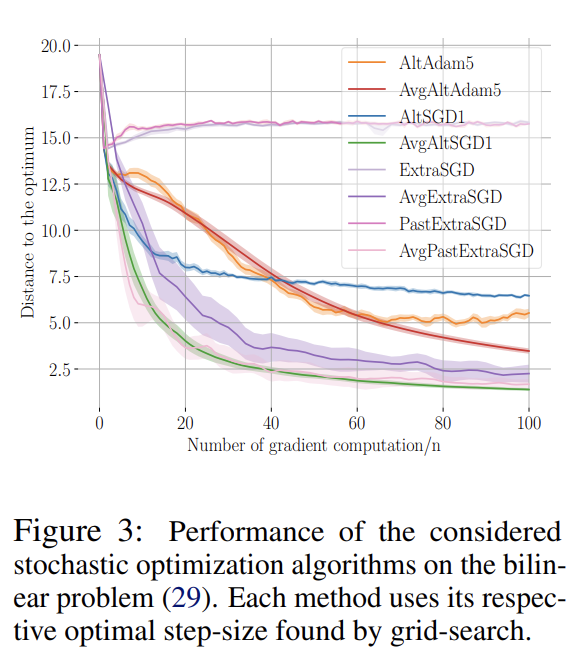
\includegraphics[scale=1]{pictures/pic3.png}
			\label{fig:la}
		\end{figure}
		\item The second test was conducted in the context of GAN training. Two different GAN architectures were used: WGAN and WGAN-GP. Only Adam version of gradient descent was evaluated. \\
		\begin{figure}[!htb]
			\centering
			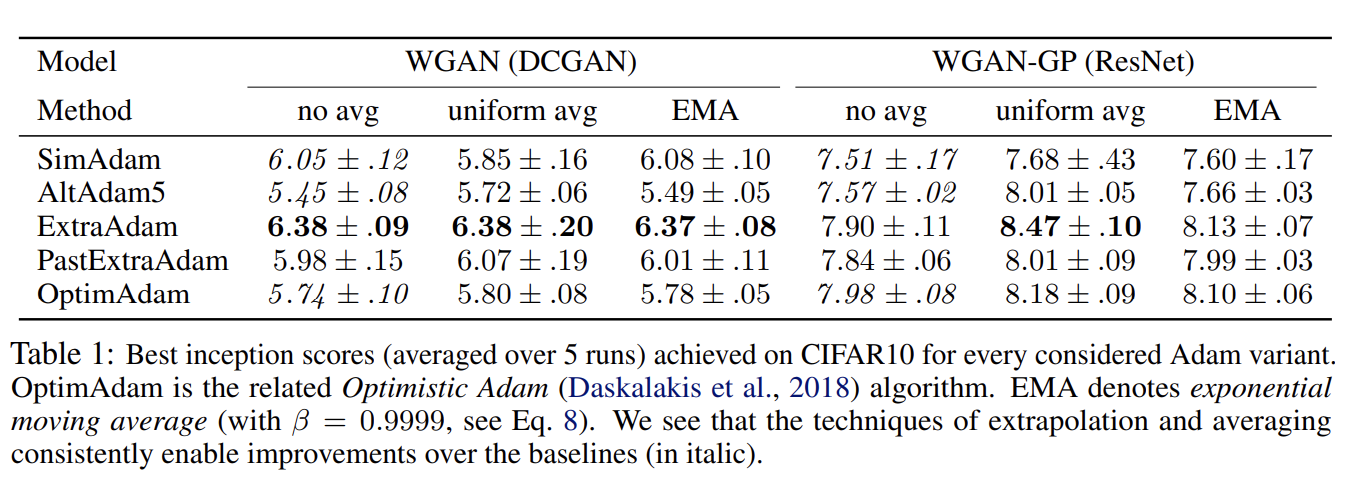
\includegraphics[scale=1]{pictures/pic4.png}
			\label{fig:lab}
		\end{figure}
		\begin{figure}[!htb]
			\centering
			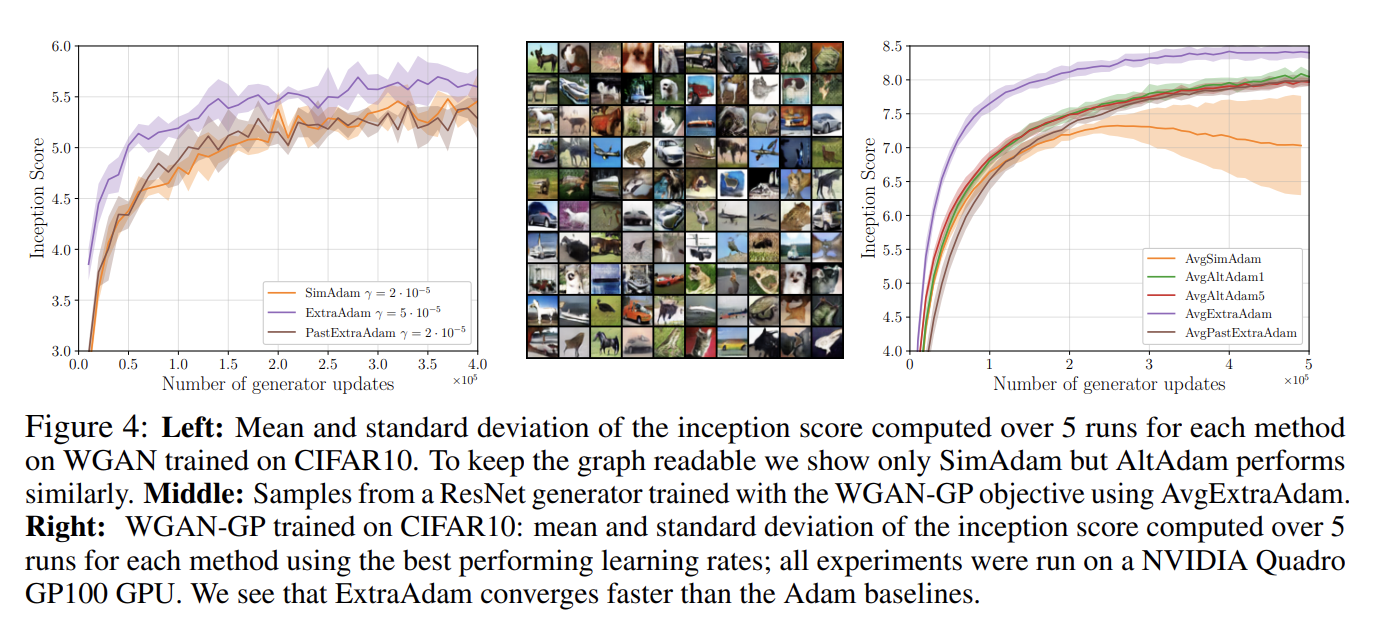
\includegraphics[scale=1]{pictures/pic5.png}
			\label{fig:l}
		\end{figure}
		
		As we can see below, for both tasks, using an extrapolation step and averaging with Adam (ExtraAdam) outperformed all other methods. Combining ExtraAdam with averaging yields results that improve significantly over the previous state-of-the-art IS and FID.
	\end{enumerate}

\section{On the Convergence of Single-Cell Stochastic Extra-Gradient Methods:}

	\subsection{Problem Statement:}
        Landscape of the loss function in GANs does not resemble the minimization problem, but that of a min-max game which in our words could be called a \textbf{variational inequality}. They have gained significant attention in machine learning, offering a flexible framework beyond ordinary loss function minimization, particularly in generative adversarial networks (GANs) and deep learning systems. The optimal $O(1/t)$ convergence rate for solving smooth monotone variational inequalities is achieved by the Extra-Gradient (EG) algorithm and its variants. These methods require two projections and two oracle calls per iteration, making them costly compared to standard methods like Forward-Backward. Reducing this cost is the main goal of the current paper.
	
	\subsection{Main Idea of the Approach:}
        The primary focus of this research is to investigate and quantify the convergence behavior of single-call stochastic extra-gradient methods when solving variational inequalities. By understanding the underlying mechanisms of these algorithms, the paper aims to provide valuable insights into their applicability and efficiency, especially in the realm of non-monotone variational inequalities.
	
	\subsection{Theory and Background: }
 
        Variational inequalities, encompassing diverse problems like minimization, saddle-points, Nash equilibria, and fixed-point problems, serve as a foundational framework in optimization. The EG algorithm, with its variants, has been pivotal in solving monotone variational inequalities. However, the computational cost involved has led to the exploration of single-call variants, sparking a significant area of research. This paper delves into these single-call methods, studying their properties and convergence rates in both deterministic and stochastic scenarios.
	
		\subsubsection{Related Work: }
  
        Existing research has explored various algorithms, such as Forward-Backward-Forward (FBF) and gradient extrapolation mechanisms like Popov's modified Arrow-Hurwicz algorithm, to reduce the number of oracle calls and projections. Among these, single-call extra-gradient methods, including Past Extra-Gradient (PEG), Reflected Gradient (RG), and Optimistic Gradient (OG), have gained prominence for their efficiency in approximating missing gradients while making a single oracle call per iteration.
		
		\subsubsection{Theoretical Framework: }
  
        In the context of variational inequalities, the Extra-Gradient algorithm involves two projections and oracle calls per iteration. Single-call variants like PEG, RG, and OG perform a single oracle call while approximating missing gradients differently. These algorithms converge at the optimal O(1/t) rate under certain assumptions.
		
		\subsubsection{Key Features: }
        \begin{itemize}
            \item Variational inequalities provide a flexible framework in machine learning beyond traditional loss function minimization.
            \item Extra-Gradient and its variants achieve optimal O(1/t) convergence rates.
            \item Single-call extra-gradient methods, such as PEG, RG, and OG, approximate missing gradients with a single oracle call per iteration.
        \end{itemize}
		
		\subsubsection{Causes behind Good Performance: }
  
        The performance of single-call extra-gradient methods is attributed to their ability to anticipate the landscape of the problem by approximating missing gradients while making only one oracle call per iteration. These methods achieve optimal convergence rates in both deterministic and stochastic variational inequalities under suitable conditions.
		
		\subsubsection{Improvements over Older Methods: }
  
        Single-call extra-gradient methods significantly reduce the computational cost associated with multiple oracle calls and projections. They retain the anticipatory properties of the original Extra-Gradient algorithm while making efficient use of oracle resources.
	
	\subsection{Essence of Proof: }
        
        The proofs for the convergence rates of single-call extra-gradient methods involve intricate analyses. Techniques such as quasi-descent inequalities and probabilistic arguments are employed to establish convergence properties. For stochastic variational inequalities, careful consideration of noise realizations and conditional bias is necessary to prove convergence rates.
	
	\subsection{Experiments and Results:}
 
        Experimental results demonstrate the efficiency of single-call extra-gradient methods in both deterministic and stochastic variational inequalities. These methods consistently outperform the traditional Extra-Gradient algorithm in terms of convergence speed, especially in scenarios where computational resources are limited.
        \begin{figure}[h]
            \centering
            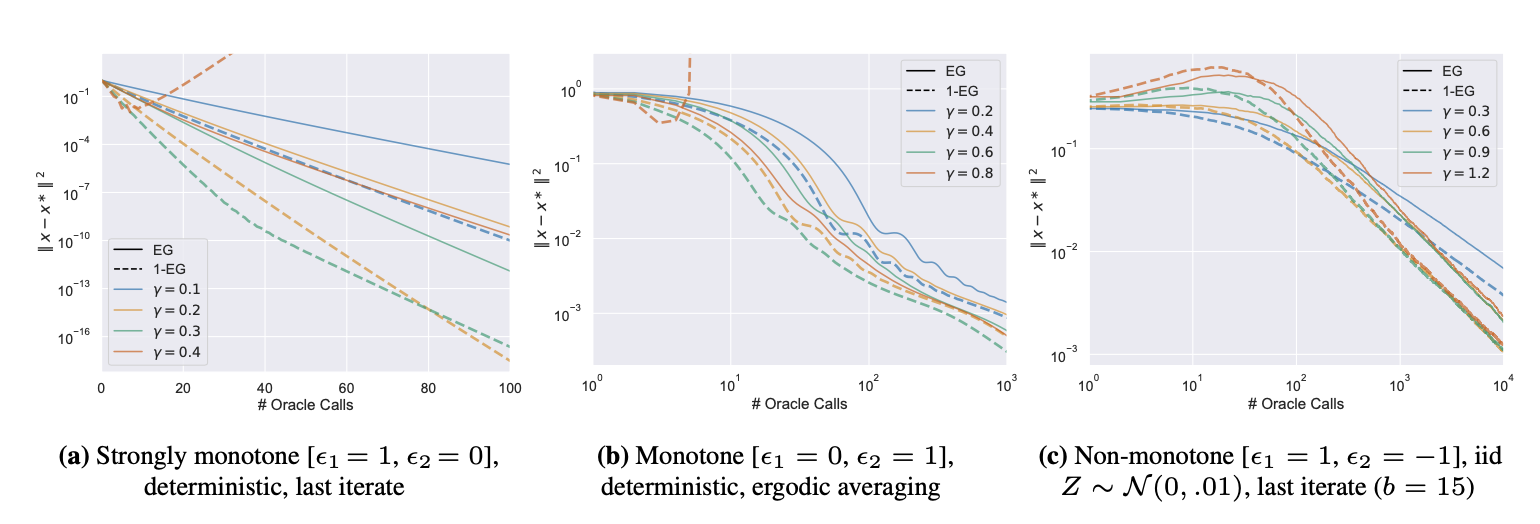
\includegraphics[scale=0.5]{pictures/pic1.png}
            \caption{Illustration of the performance of EG and 1-EG in the (a priori non-monotone) saddle-point problem $\mathcal{L}(\theta, \phi) = 2 \epsilon_1 \theta^T A_1 \theta + \epsilon_2 (\theta^T A_2 \theta)^2 - 2 \theta_1 \phi^T B_1 \phi - \epsilon_2 (\phi^T B_2 \phi)^2 + 4\theta^T C \phi$ }
            \label{fig:label}
        \end{figure}
 
	
\section{Conclusion:}
	Both techniques that we have covered have used theoretical transformation of the problem to variational inequality problem, and then focused on optimizing the objective in the new terms. Both of them have managed to achieve better computational efficiency than older algorithms, and achieved best results during the evaluation. Both of the papers focused on this problem in order to improve GAN training. However, the experimentation of the authors of the first paper was more rigorous - more expansive tests were conducted using different settings to prove that their method works well.
\end{document}